\section{Methods}
\label{sec:methods}

\subsection{Overview}
Figure~\ref{fig:concept} illustrates the idea. The wind measured at a reference station is first converted to the wind at the height of the roadside sensor over open terrain, then corrected for the roughness around both sites and for the persistent exposure of the reference station, and finally for the shelter of the road corridor; the estimates of all reference stations are then combined. For a roadside station $j$ and a reference station $s$ the hourly wind speed is transferred in four steps,
\begin{equation}
U_0 \xrightarrow{\text{height}} U_1 \xrightarrow{\text{roughness}} U_2 \xrightarrow{\text{site factor}} U_3 \xrightarrow{\text{roadside exposure}} U_4 ,
\label{eq:ladder}
\end{equation}
and the estimates from all reference stations are combined (Section~\ref{sec:combine}). Direction-dependent quantities are evaluated in the 16 sectors of the wind-from direction of the vector-mean wind of the reference network, $k(t)$. Each step is evaluated separately, so that its contribution to the error reduction can be read directly. The same model, with the same predictors, is fitted separately in each country.

\begin{figure}[!htbp]
\centering
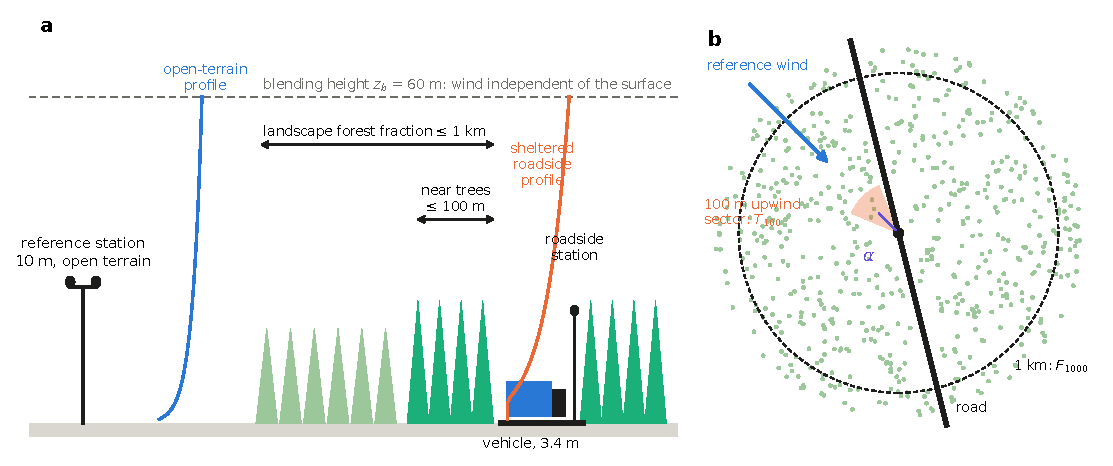
\includegraphics[width=\textwidth]{figures/fig00_concept.pdf}
\caption{The problem and the predictors. (a) Side view: the reference station measures over open terrain at \SI{10}{m}; above the blending height the wind is independent of the surface; at the road, trees next to the road and the forest of the surrounding landscape reduce the wind at the roadside sensor and at the vehicle. (b) Plan view of the exposure predictors at a roadside station: the near-tree share $T_{100}$ in the upwind sector within \SI{100}{m}, the forest fraction $F_{1000}$ within \SI{1}{km} in all directions, and the angle $\alpha$ between the reference wind and the road axis, which controls the deflection of the wind direction. Schematic, not to scale.}
\label{fig:concept}
\end{figure}

\subsection{Height conversion}
Under neutral stratification over open terrain ($z_{0r}=\SI{0.03}{m}$),
\begin{equation}
U_1 = U_0\,\frac{\ln(z_j/z_{0r})}{\ln(z_s/z_{0r})},
\end{equation}
with $z_s=\SI{10}{m}$; $z_j=\SI{6}{m}$ in Sweden (factor 0.912) and $\SI{10}{m}$ in Norway (factor 1). The same open-terrain profile converts every wind to vehicle height, $z=\SI{3.4}{m}$ (factor 0.814 from \SI{10}{m}); Section~\ref{sec:energy-method} gives the sensitivity of the results to this choice.

\subsection{Roughness conversion}
Following \citet{Wieringa1986}, the wind at a blending height $z_b=\SI{60}{m}$ is assumed to be independent of the local surface. The measured wind is converted to the potential wind over open terrain and then to the roadside,
\begin{align}
G_s(z_0) &= \frac{\ln(z_b/z_0)}{\ln(z_s/z_0)}\,\frac{\ln(z_s/z_{0r})}{\ln(z_b/z_{0r})}, \qquad
G_j(z_0) = \frac{\ln(z_b/z_{0r})}{\ln(z_s/z_{0r})}\,\frac{\ln(z_j/z_0)}{\ln(z_b/z_0)},\\
U_2 &= U_0\,G_s\!\left(z_{0,s}(k)\right)\,G_j\!\left(z_{0,j}(k)\right).
\end{align}
The effective roughness length in sector $k$ is a footprint-weighted geometric mean over the \SI{10}{m} pixels within $\pm\ang{22.5}$ of the upwind direction, with weights $e^{-r/L}$, $L=\SI{100}{m}$, and $z_{0}=0.1\,h$ where the object height $h>\SI{5}{m}$, \SI{0.0002}{m} over water and $z_{0r}$ elsewhere. No zero-plane displacement is used: the roadside sensors stand in clearings and corridors, below or at the height of nearby canopies, where the logarithmic profile does not strictly hold \citep{Raupach1994,Finnigan2000}; the conversion is therefore a first-order correction whose residual is left to the empirical exposure model.

\subsection{Site factors of the reference stations}
Each reference station has a persistent exposure that the roughness conversion captures only partly (coast, hill tops, valleys, nearby obstacles). On the training period the potential wind is decomposed as
\begin{equation}
\ln U_{\mathrm{pot},s}(t) = a(t) + c_s + \varepsilon_{s}(t),\qquad \sum_s c_s=0,
\end{equation}
where $a(t)$ is the network-common term of hour $t$ and $c_s$ the site factor of station $s$, fitted by alternating least squares on hours with a network median speed $\ge\SI{3}{m.s^{-1}}$ and at least 12 reporting stations. The corrected wind is $U_3 = U_2\,e^{-c_s}$. Direction-dependent site factors were tested and did not improve the result (Section~\ref{sec:res-sens}).

\subsection{Roadside exposure model}
The remaining ratio between the roadside observation and $U_3$ is modelled as
\begin{equation}
\ln\frac{U_j}{U_3} = b_0 + b_1\,T_{100}(k) + b_2 \ln\frac{x}{h}(k) + b_3 \ln U_{\mathrm{net}} + b_4\,F_{1000} + \varepsilon ,
\label{eq:exposure}
\end{equation}
where $T_{100}$ is the fraction of pixels with objects $>\SI{5}{m}$ within \SI{100}{m} upwind ($\pm\ang{22.5}$), $F_{1000}$ the same fraction within \SI{1}{km} in all directions (the forest fraction of the landscape), $x/h$ the distance to the first upwind obstacle divided by its height (median over seven rays in the sector, capped at \SI{1500}{m}) and $U_{\mathrm{net}}$ the mean site-corrected wind of the reference network. The model is fitted by ordinary least squares on station pairs and hours with $U_0\ge\SI{2}{m.s^{-1}}$, a roadside speed above \SI{0.2}{m.s^{-1}} and all predictors available; the back-transformation uses the smearing estimate \citep{Duan1983}, computed without the predicted roadside station. The form of Eq.~\eqref{eq:exposure} results from the selection described in Section~\ref{sec:validation}.

\subsection{Wind direction}
Road corridors deflect the wind towards the road axis. With $\alpha$ the angle between the reference wind direction and the road axis,
\begin{equation}
\varphi_j = \varphi_s + d_0 + d_1 \sin(2\alpha)\,T_{200},
\end{equation}
a form analogous to the terrain-diverting factor of \citet{ListonElder2006}, fitted by least squares on the wrapped direction difference in hours with $U_0\ge\SI{3}{m.s^{-1}}$ and a roadside speed of at least \SI{1.5}{m.s^{-1}}.

\subsection{Combination of the reference stations}
\label{sec:combine}
The roadside wind speed is the weighted geometric mean of the estimates $U_{4,i}$ from all reference stations within \SI{150}{km} (\SI{120}{km} in Norway), with weights $w_i = d_i^{-1.5}$ ($d_i$ distance, floored at \SI{3}{km}); the direction is the weighted vector mean from stations within \SI{60}{km} ($w_i=d_i^{-1}$; the nearest station if none is within \SI{60}{km}).

\subsection{Comparison estimators}
\label{sec:baselines}
The corrected estimate is compared with four alternatives that need no exposure model. \emph{Nearest station}: the nearest reference station with data in the hour, converted to the sensor height. \emph{Rescaled nearest station}: the same multiplied by one constant, the ratio of the mean roadside to the mean nearest-station wind, learned on the other time blocks and the other roadside stations. \emph{Nearest road station}: the wind of the nearest other road weather station with speed and direction in the hour; this is what a practitioner with access to the road weather network would use. \emph{MET Nordic}: the analysis interpolated to the station (Section~\ref{sec:data}). All estimators are scored on the same hours. Because the exposure model is fitted in log space, its estimate can be conditionally biased; a recalibrated variant multiplies it by the ratio of the mean observed to the mean estimated wind in bins of the estimate, again learned on the other blocks and stations.

\subsection{Validation design}
\label{sec:validation}
Parameters are never evaluated on the data used to fit them. The test period is divided into consecutive time blocks---eight blocks of about three months in Norway, so that every season is left out once, and four blocks of about three days in Sweden. The exposure and direction models are fitted on all blocks but one and on all roadside stations except the one predicted (leave-one-station-out, LOSO), and evaluated on the remaining block; every prediction is therefore out of time and out of station \citep{Roberts2017}. Site factors are estimated only from the year before the test period. The score is the mean absolute error (MAE) of the hourly wind speed per roadside station, summarised by the median over stations; two settings are compared with paired differences per station and their standard error (SE). The bias is reported as the ratio of the mean estimated to the mean observed wind speed minus one, over all hours with both values. Uncertainty across stations is given as 95\,\% intervals from a station-cluster bootstrap (2000 resamples of stations); it is the relevant uncertainty because the exposure predictors vary only between stations and sectors.

The predictors and the form of the station combination were chosen on the Swedish record (\ref{app:sweden}) and then fitted anew in Norway. Length scales and thresholds were varied one at a time; a value is retained when it is within one standard error of the best value of its group \citep{Hastie2009}, preferring the physically better founded or simpler one. Because these choices were scored with the same cross-validation that is reported, all Norwegian choices were also repeated on 2024 alone (four blocks), and the resulting model, fitted on 2024, was evaluated leave-one-station-out on the untouched year 2025. Terrain indices from the Norwegian terrain model---the upwind shelter index $S_x$ \citep{Winstral2002} within \SI{300}{m} and \SI{1}{km}, the topographic position index within \SI{500}{m} and \SI{2}{km}, and the relief within \SI{2}{km}---were tested as additional predictors of the final model.

\subsection{Transfer between the countries}
To test whether the fitted model can be used in a region without roadside stations, the coefficients of Eq.~\eqref{eq:exposure} and of the direction model fitted in one country are applied unchanged in the other; the physical steps and the site factors use the local data.

\subsection{Application at vehicle height}
For the NOR-XWIND segments, the model fitted on all Norwegian roadside data is applied with the segment's own features and the reference observations of the hour nearest to the passage. It predicts the wind that a \SI{10}{m} roadside anemometer at the segment would measure; this is converted to \SI{3.4}{m} with the same open-terrain factor as all other estimates (sensitivity: the local-$z_0$ profile). It is compared with no wind, the nearest reference station and the nearest road weather station, both converted in the same way, and with the MET Nordic analysis at \SI{10}{m}, converted in the same way. Because the station-based estimates are hourly, results are averaged per reference hour, and intervals are obtained by resampling hours.

\subsection{Air drag and energy}
\label{sec:energy-method}
Wind is propagated to the air drag of a tractor--semitrailer with
\begin{align}
F_D &= \tfrac12 \rho\, C_dA(\beta)\, v_a^2, & v_a^2 &= (v_v+v_{wx})^2+v_{wy}^2, & \beta &= \arctan\frac{|v_{wy}|}{v_v+v_{wx}},
\label{eq:drag}
\end{align}
with the vehicle speed $v_v$, the head- and crosswind components $v_{wx}$ (positive against the direction of travel) and $v_{wy}$, the air speed $v_a$, the yaw angle $\beta$ and $\rho=\SI{1.25}{kg.m^{-3}}$. The drag area at zero yaw is $C_dA(0)=\SI{5.8}{m^2}$, the typical value certified for EU 4$\times$2 long-haul tractor--trailers \citep{ICCT_VECTO}. Its yaw dependence follows the generic speed-dependent crosswind correction for tractor--semitrailers of VECTO, the simulation tool of the EU certification of heavy-duty vehicles \citep{EU2017_2400,VECTO},
\begin{equation}
C_dA(\beta) = C_dA(0) + a_1\beta + a_2\beta^2 + a_3\beta^3,
\label{eq:vecto}
\end{equation}
with $a_1=0.030042$, $a_2=0.040817$, $a_3=-0.002130$, $\beta$ in degrees and $C_dA$ in \si{m^2}, held constant beyond its maximum at $\beta=\ang{13.1}$ (a 45\,\% increase), which is exceeded in \enCapPctNo\,\% of the passes. As an upper bound of the crosswind sensitivity we also use Model~1 of \citet{Askerdal2024crosswind}, $C_dA(\beta)\propto\cos^2\beta\,(A_f\cos\beta+A_s\sin\beta)$ with $A_f=\SI{10.3}{m^2}$ and $A_s=\SI{57.6}{m^2}$, scaled to the same $C_dA(0)$; it nearly doubles the drag area at \ang{10} yaw, where Eq.~\eqref{eq:vecto} gives \SI{39}{\percent}.

The energy needed to overcome air drag per distance equals the force; we report it in \si{kWh} per \SI{100}{km} at the wheel. At each roadside station with adequate direction coverage and each hour a vehicle is driven in both directions along the road axis at \SI{80}{km.h^{-1}} (sensitivity: 60--\SI{90}{km.h^{-1}}); a round trip is the mean of both directions. The results therefore describe the station sites, which are not a random sample of the road network. All winds---observed and estimated---are referred to vehicle height (\SI{3.4}{m}) with the same open-terrain factor, so that this conversion does not favour any estimator. We define the wind penalty as the air-drag energy with wind minus that in still air, relative to the still-air energy; it does not depend on the air density, whose range in the region (about 1.15--\SI{1.32}{kg.m^{-3}} between warm lowland and cold mountain conditions) changes the absolute energy by $-8$ to $+6$\,\% relative to the value of \SI{1.25}{kg.m^{-3}} used here. Head/tail-only and crosswind-only penalties are computed with one wind component set to zero; because Eq.~\eqref{eq:drag} is not additive in the components, they do not sum exactly to the total.

The size of the penalty depends on assumptions that cannot be checked with the roadside data. Its uncertainty is explored by repeating the calculation with the observed wind and (i) a sensor height of \SI{6}{m} instead of \SI{10}{m}; (ii) roughness lengths of 0.01--\SI{0.3}{m}, with and without a displacement height of \SI{2}{m}, and no height reduction at all for the profile from \SI{10}{m} to \SI{3.4}{m}; (iii) Model~1 instead of the VECTO curve; and (iv) a turbulence correction, averaging Eq.~\eqref{eq:drag} over Gaussian longitudinal and lateral fluctuations of the wind with standard deviations $\sigma_u=I\,U$ and $\sigma_v=0.8\,\sigma_u$, $I=0.15$ and $0.3$, a simple form of the wind-averaged drag \citep{Windsor2014,WordleySaunders2008}.

The estimators of Section~\ref{sec:baselines}, and no wind (common practice in range prediction), are compared by the mean absolute error of the hourly one-way energy, its skill score $1-\mathrm{MSE}/\mathrm{MSE}_\text{no wind}$, the long-term penalty of each station site (mean over all hours and both directions) and its correlation with the observed penalty, and the error in hours with a substantial wind effect, in which the observed wind changes the air-drag energy by at least \SI{10}{\percent}. Intervals are from the station-cluster bootstrap. For the vehicle segments, the energy is evaluated along the measured heading.
